\subsection{flowws}
In den zwei vorangegangenen Kapiteln wurden die zwei Paradigmen beschrieben, welche die Anforderungen bezüglich des Programmiermodells erfüllen sollen, namentlich die sequentielle und parallele Programmierung der cBlocks in visueller Form. Im Folgenden wird das Zusammenspiel beider Paradigmen erklärt. Dabei wird auf das Konzeptmodell, Ausführungsmodell und die Eigenheiten von flowws bezüglich des cBlocks-Kontext eingegangen. Dieses Modell inklusive der visuellen Darstellung sind die Bestandteile der \ac{EUD} flowws.

\begin{figure}[h]
  \centering
  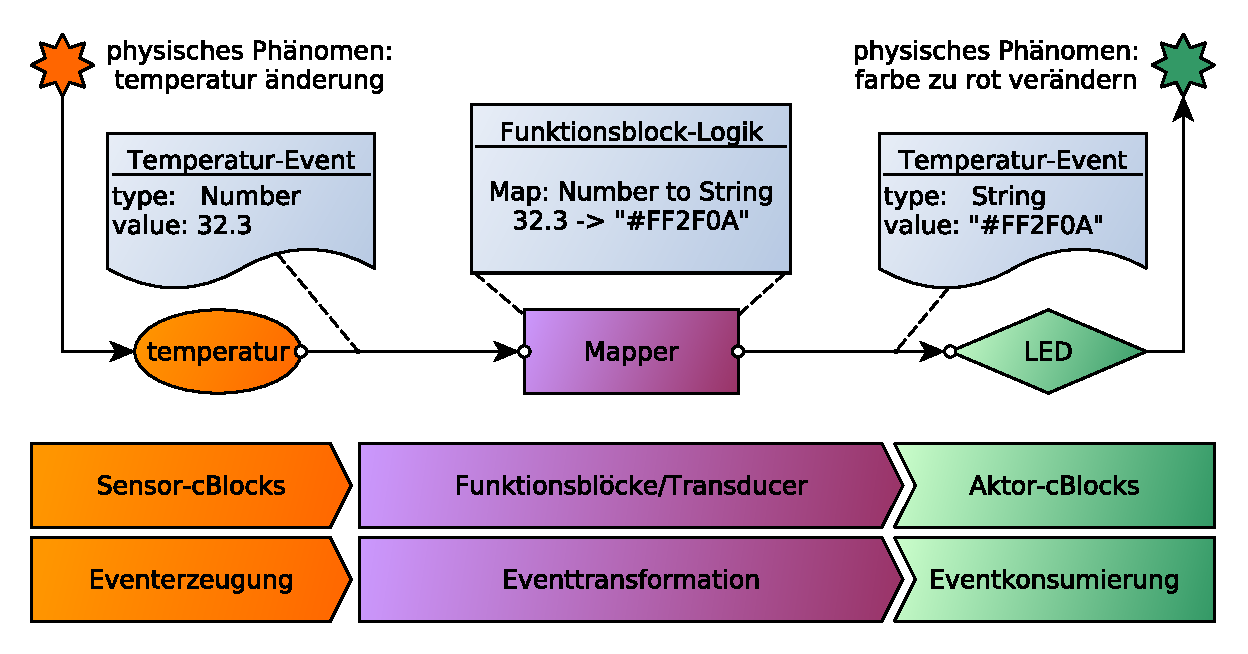
\includegraphics[width=1\textwidth]{bilder/chapter4/chapter4_2/flowwsschematicexample.pdf}
  \caption{Ein schematisches Beispiel für das Ausführungsmodells von flowws. Die Daten fließen von der Erzeugung als Events durch Funktionsblöcke um zu transformiert zu werden. Dadurch erhalten sie einen höheren semantischen Wert, sodass sie vom Aktor konsumiert werden können.}
  \label{fig:beispielflowws}
\end{figure}

In Abbildung \ref{fig:beispielflowws} word ein in flowws modelliertes Programm schematisch dargestellt.  Im Beispiel wird von einem Temperatur-Sensor ein Temperatur-Event erzeugt, welches die Farbe der LED manipulieren soll (blau für kalt, rot für warm). Hierbei wird ein Funktionsblock verwendet, der den \texttt{Number}-Wert des Events auf eine Wertebereich von Farben abbildet. Dieses semantisch höherwertige Event wird dann vom Aktor bzw. der \ac{FSM} des Aktors verwendet, um dessen Zustand zu ändern. Hierbei wird das Kernprinzip von flowws, das sich in in drei Schritte aufteilt, verdeutlicht:

\subsubsection{1. Eventerzeugung}
 Eventerzeugung ist die erste Phase jedes flowws-Programmes. Jeder Sensor-cBlock, der mit dem System verbunden sind, besitzt einen virtuellen Sensorblock als Repräsentant. Jeder Sensorknoten entspricht einem cBlock, d.h. cBlocks, welche mehrere unterschiedliche Events erzeugen (bspw. ein cBlock der Temperatur und Luftfeuchtigkeit misst) werden als einen Knoten mit mehreren Ausgängen dargestellt. 
 
 Wie in Abbildung \ref{fig:seqsensorblock} gezeigt, erzeugen Sensorblocks kontinuierlich Events mit Rohdaten als \textit{Payload}, auf Basis physikalischer Phänomene. Diese Rohdaten haben oftmals keine semantische Bedeutung und sind in vielen Fällen schlichtweg Zahlenwerte oder Zeichenketten (siehe Tabelle \ref{tab:datentypenpayloads}).
 
 \begin{figure}[h]
  \centering
  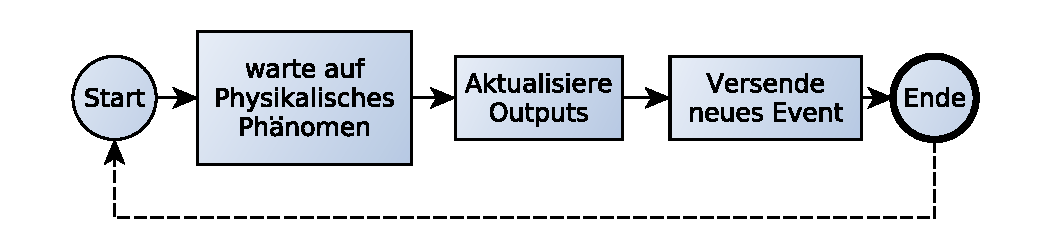
\includegraphics[width=1\textwidth]{bilder/chapter4/chapter4_2/sensorblockablauf.pdf}
  \caption{Standardablauf innerhalb eines Sensorblocks, wenn ein physikalisches Ereignis erfolgt ist.}
  \label{fig:seqsensorblock}
\end{figure}

 Wie alle anderen Knoten innerhalb von flowws sind auch Sensorknoten \textit{Black Boxen}. Der Unterschied zu anderen Knoten ist allerdings, dass sie keine Eingänge besitzen, sondern nur Ausgänge als Schnittstellen, da sie selbst nicht in ihrem Verhalten beeinflusst werden sollen. Dies soll die Verbindung zum physikalischen Sensor cBlock stärken, da es intuitiv ist, dass Aktoren ein aktives Verhalten aufzeigen während Sensoren passiv ihre Umgebung wahrnehmen. 
 
 \subsubsection{2. Eventtransformation}\label{subsubsec:eventtrans}
 Bei der Eventtransformation kommt dass \ac{DBP}-Paradigma aus Kapitel \ref{subsection:datenflussprog} zu tragen. Die erzeugten Daten werden durch eine Reihe von Funktionsblöcke geleitet und somit miteinander kombiniert und/oder transformiert. 
 
 Der Ablauf einer Transformation in einem Funktionsblock ist in Abbildung \ref{fig:seqfunktionsblock} dargestellt.
 \begin{figure}[h]
  \centering
  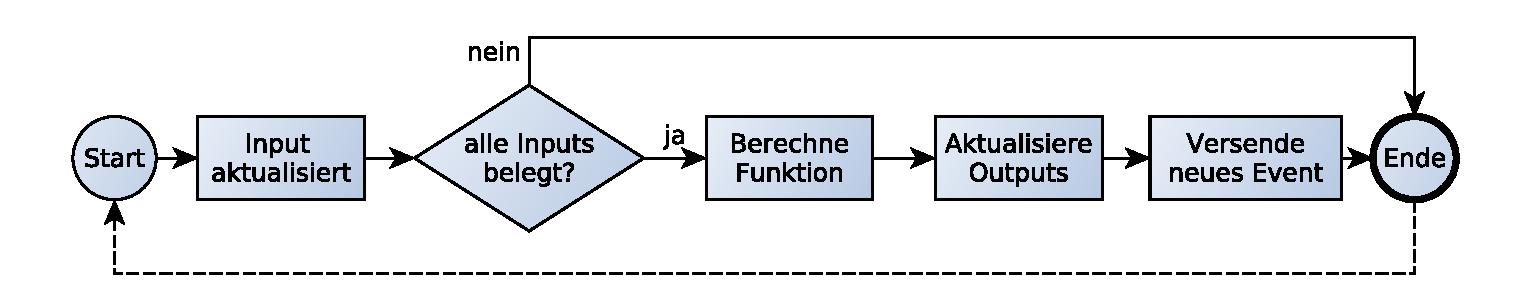
\includegraphics[width=1\textwidth]{bilder/chapter4/chapter4_2/funktionsblockablauf.pdf}
  \caption{Standardablauf innerhalb eines Funktionsblocks, wenn eine Input-Schnittstelle aktualisiert wird.}
  \label{fig:seqfunktionsblock}
\end{figure}
Wenn sich eine Input-Schnittstelle durch ein eintreffendes Ereignis aktualisiert wird, prüft der Transducer nach, ob sämtliche Input-Schnittstellen einen Wert besitzen. Der Block nimmt dann seine Transformation der Events vor, gibt das Ergebnis an die Output-Schnittstellen weiter, welche das neue Ereignis versenden. Folgendes ist hierbei zu beachten: 
\begin{itemize}
    \item Eingehende Signale werden nicht wie bei \ac{DBP} üblich, in der Input-Schnittstelle in einer \textit{Queue} gepuffert und nacheinander abgearbeitet, sondern überschrieben. Der Grund hierbei ist, dass cBlocks zu jeder Zeit auf den momentanen Zustand ihrer Umgebung reflektieren sollen. Zum Beispiel macht es wenig Sinn, nicht mehr aktuelle Umgebungstemperaturen nacheinander abzuarbeiten.
    \item Events werden von Funktionsblöcken nicht konsumiert. Aufgrund der gleichen Rationale wie der vorherige Punkt, sollen die Events immer den momentanen Zustand der physischen Umgebung widerspiegeln, in der sich die (physischen) cBlocks befinden. Gibt es bspw. mehrere Sensoren mit unterschiedlichen Abtastfrequenzen müssen sämtliche Signale immer auf das Signal des Langsamsten warten. In solchen Fällen wird das letzte Signal als das Aktuellste betrachtet und zur durchführung der Funktion verwendet.
\end{itemize}
 Die Funktionen zur Transformation von Ereignissen, orientieren sich an den funktionalen Anforderungen FA\#1 bis FA\#6:
 \begin{itemize} 
     \item Bei \textbf{Bool'sche Gattern} handelt es sich um logische Operationen, die auf ein oder mehrere bool'sche Signale angewandt werden. Zu den Funktionen zählen: Negation, logisches Und/Oder und exklusives Oder ($\neg, \land, \lor, \oplus$). Sie überprüfen den Ausdruck abhängig der Eingänge auf Wahrheit und geben das bool'sche Ergebnis weiter.
     \item Zu \textbf{Vergleichsoperationen} gehören sämtliche Operationen, die zwei Zahlen miteinander vergleichen können, und einen bool'schen Wert ausgeben ($<,\leq,=,\neq,\geq,>$).
     \item \textbf{Zeitgesteuerte Operationen} erlauben es dem Nutzer Signale auf ihre temporären Eigenschaften zu manipulieren d.h. Signale zeitlich zu verzögern oder Signale periodisch zu wiederholen.
     \item \textbf{Konvertierungsoperationen} wandeln Signale um, indem sie den Wertebereich des Eingangssignals auf einen vordefinierten Zielbereich des Ausgangssignals zuweisen. Dies kann auf zwei weisen geschehen: kontinuierliche Wertebereiche ([1,2,3,..,n] -> [-n,...,-3,-2,-1]) oder kategorische Wertebereiche ([<=30,>30] -> [kalt,heiß])
     \item Der \textbf{Generische Operator} erlaubt es Experten ihre eigenen Transformationen in Programmcode zu beschreiben. Dieser Programmcode kann beliebig viele Ein- und Ausgänge besitzen sowie ein beliebige Kombination von Datentypen, solange sie mit denen von Tabelle \ref{tab:datentypenpayloads} übereinstimmen
 \end{itemize}
 Es können noch weitere vorgefertigte Funktionen definiert werden, allerdings würde dies den Rahmen dieser Arbeit hinausgehen und wäre nicht Zielführend, führ die Definition einer \ac{EUD}. Durch Funktionsblöcke mit selbstdefinierter Logik wird allerdings Funktionsblock vorgesehen, der es dem Endnutzer erlaubt, eigene Transformationslogik einzuprogrammieren und somit der \ac{EUD} erlaubt, jede beliebige Funktion ab zu bilden.
 
\subsubsection{3. Eventkonsumierung} \label{subsubsec:evebtkonsumierung}
Mit dem Konsumieren der Events schließt sich der Kreis indem ein initiales physisches Phänomen, dass durch die Sensor-cBlocks aufgenommen wurde in einem neuen physischen Phänomen, dass vom Aktor-cBlock erzeugt wird (siehe Abbildung \ref{fig:beispielflowws}). 

Jeder Aktor-cBlock, der mit flowws verbunden wird, ist ähnlich wie bei den Sensor-cBlocks mit einer virtuellen Abbild (hier Aktorblock) repräsentiert. Ein Aktorblock ist intern eine \ac{FSM} wie sie in Kapitel \ref{subsec:fsmprogrammierung} beschrieben. Hierbei werden vom Endnutzer Zustände, Übergänge und Übergangslogik definiert um dem Aktor ein gewünschtes Verhalten zu verabreichen.

 \begin{figure}[h]
  \centering
  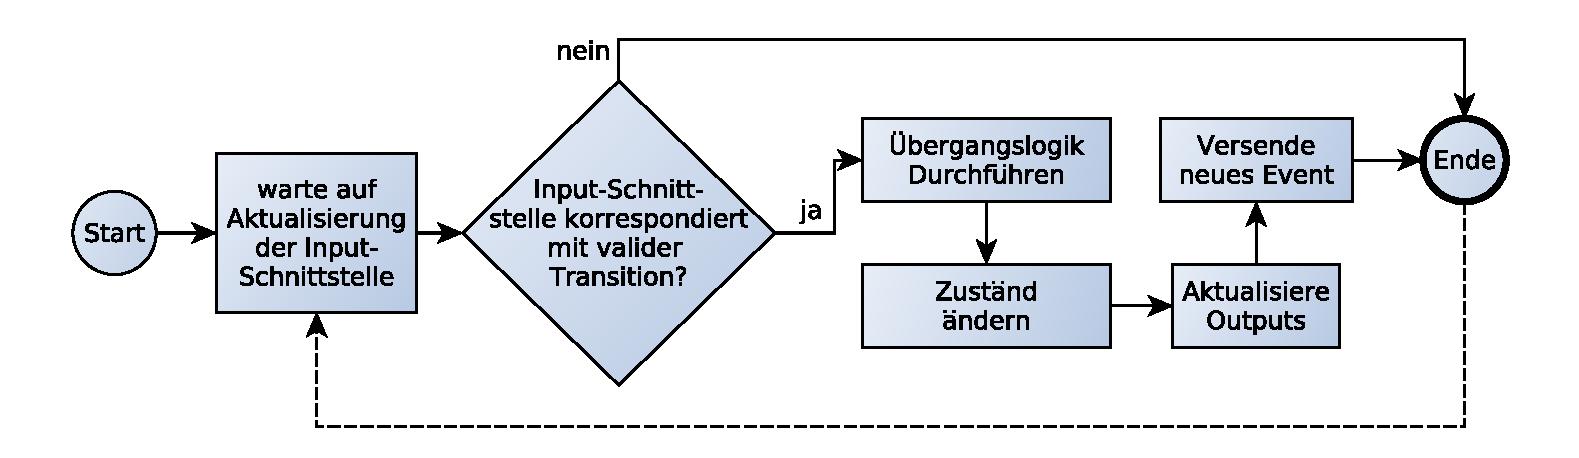
\includegraphics[width=1\textwidth]{bilder/chapter4/chapter4_2/aktorblockablauf.pdf}
  \caption{Standardablauf innerhalb eines Aktorblocks, wenn eine Input-Schnittstelle aktualisiert wird.}
  \label{fig:seqfunktionsblock}
\end{figure}

In Abbildung \ref{fig:seqfunktionsblock} ist der Ablauf zu sehen, der Durchgeführt wird, sobald ein neues Event eintrifft. Zuerst ermittelt der Aktorblock mit welcher Transition die aktualisierte Input-Schnittstelle korrespondiert. Als Nächstes wird überprüft ob die Transition valide bzw. erlaubt ist abhängig von dem Zustand, indem sich der Aktorblock momentan befindet. Ist dies der Fall, wird die Übergangslogik ausgeführt und abhängig davon, des Events und der Aktorfunktionen die Eigenschaften des Aktors verändert. Hierdurch wird ein physikalisches Signal erzeugt. Ebenso kann optional ein neues Signal erzeugt werden und über eine Output-Schnittsstelle, welches auch mit der Überganglogik korrespondiert, versendet werden. Ein Aktorblock ist somit mehr als nur ein Konsument; er kann ebenso wie ein Sensorblock neue Signale erzeugen, welche wiederum transformiert und von weiteren Aktorblocks konsumiert werden können.

Jeder Aktorblock besitzt zusätzlich zu seiner \ac{FSM} zwei weitere Komponenten:
\begin{itemize}
    \item \textbf{Aktoreigenschaften} sind alle Eigenschaften, welche die Art des physikalische Signals beeinflussen. Ein LED-cBlock kann die Aktoreneigenschaften \texttt{(r,g,b)} und \texttt{(Brightness)} besitzen; ein Lautsprecher-cBlock kann die Eigenschaften \texttt{(AudioFrequency)} und \texttt{(Loudness)} besitzen oder ein LCD-cBlock kann die Eigenschaft \texttt{(DisplayText)} besitzen. Vorgegeben werden diese Eigenschaften von dem cBlocks \textit{Back-end}. Auf Hardwareebene werden solche Aktoreneigenschaften als \textbf{Ressource} bezeichnet. Von diesem abstrakten Begriff wird aufgrund von Benutzerfreundlichkeit allerdings in flowws Abstand genommen.
    \item \textbf{Aktorfunktionen} sind Aktionen der einzigste Weg innerhalb von flowws Aktoreigenschaften direkt zu manipulieren. Jeder Aktorblock wird mit einem Menge von Funktionen geliefert. Diese bestehen aus Funktionen wie \texttt{setColor()}, \texttt{setBrightness()}, \texttt{setFrequency()}, etc; und ermöglichen dem Endnutzer den Aktor durch geschickte modellierung der Übergangslogik zu manipulieren. Anders als die Aktoreigenschaften kann ein Experte zusätzliche Funktionen hinzufügen und somit die Flexibilität von Aktoren bei der Manipulation ihrer Eigenschaften erhöhen.
\end{itemize}

\subsubsection{Zusammenfassung}
Hiermit wurde das Programmiermodell von flowws geklärt, eine Fusion von \ac{DBP} und \ac{FSM}. Es handelt sich hierbei um eine neues Programmiermodell, welches aus diesem Grund noch nicht als \ac{EUD} verwendet wurde. Deshalb kann noch keine objektive Aussage über die Effektivität des Modells hinsichtlich Benutzerfreundlichkeit gemacht werden. Nichts desto trotz kann man die erhofften Vorteile logisch schlussfolgern:

\begin{itemize}
    \item \textbf{Leicht Erlernbar:} Das Modell basiert auf \ac{DBP} und \ac{FSM}. Beides sind Konzepte die in der Informatik und Elektrotechnik weite Verbreitung finden. Diese Beliebtheit haben beide Konzepte ihrer Fähigkeit schwere Konzepte (Parallelität und \textit{State-Management}) intuitiv darzustellen zu verdanken. Zusätzlich sind Konzepte wie \ac{DBP} und \ac{FSM} auch in verschiedenen Werkzeugen die häufig von Designern verwendet werden (bspw. \textit{Game Engines} und 3d Modellierungs Software). Es besteht also eine gute Chance, dass auch nicht Experten die Konzepte von flowws schnell erlernen können.
    \item \textbf{Leichter Verständlich:} \ac{DBP} und \ac{FSM} besitzten pendants in der UML. Es lassen sich deshalb beide Teile die als Ganzes flowws ergeben gut graphisch Darstellen. Die bildliche Darstellung sollte eine bessere Verständlichkeit über die Vorgänge innerhalb des Programmes führen und somit etwaige Fehlersuche beschleunigen.
    \item \textbf{Flexibel:} flowws bringt mit Funktionsblöcken und Aktorfunktionen viel vorgefertigte Programmlogik mit. Allerdings können beide Elemente auch durch Experten erweitert werden um flowws optimal auf den Anwendungsfall anzupassen.
    \item \textbf{Sequentiel vs. Parallel Problem:} Das Problem aus Kapitel \ref{sec:problemanalyse} wurde durch die Kombination von \ac{DBP} und \ac{FSM} beseitigt.
\end{itemize}

Im nächsten schritt wird die graphische Oberfläche und Darstellung der einzelnen elemente sowie die Interaktionen mit ihnen geklärt.